\documentclass{article}
\usepackage{amsmath} %This allows me to use the align functionality.
                     %If you find yourself trying to replicate
                     %something you found online, ensure you're
                     %loading the necessary packages!
\usepackage{amsfonts}
\usepackage{lineno}
\linenumbers
\usepackage[margin=1.0in]{geometry}
\usepackage{float}
\usepackage{graphicx}
\usepackage{multicol}
\newcommand{\nCr}[2]{\,_{#1}C_{#2}} % nCr
\newcommand{\nPr}[2]{\,_{#1}P_{#2}} % nPr
\usepackage{natbib}        %For the bibliography
\bibliographystyle{apalike}%For the bibliography
\usepackage{Sweave}
\begin{document}
\Sconcordance{concordance:exam22.tex:exam22.Rnw:%
1 16 1 1 0 355 1 1 3 5 0 1 2 10 1 1 2 4 0 1 2 4 1 1 5 4 0 1 7 5 0 1 3 5 %
0 1 3 8 1 1 5 4 0 1 2 1 0 1 2 4 0 1 2 2 1 1 3 9 0 1 2 4 1 1 2 1 0 1 1 3 %
0 1 2 1 10 2 1 1 14 1 2 19 1 1 20 1 3 1 5 4 0 1 1 9 0 1 2 17 1 1 2 1 0 %
2 1 9 0 1 1 9 0 1 2 11 1 1 2 10 0 1 2 6 1 1 22 1 2 1 6 5 0 1 1 10 0 1 2 %
19 1 1 2 1 0 2 1 10 0 1 1 10 0 1 2 13 1 1 2 10 0 1 2 6 1 1 21 2 2 32 0 %
1 1 7 0 1 2 4 1 1 12 20 0 1 2 4 1 1 4 3 0 1 1 9 0 1 2 4 1 1 3 2 0 1 3 5 %
0 1 2 1 4 11 0 1 2 6 1 1 22 1 2 1 3 2 0 1 1 8 0 1 2 19 1 1 2 1 0 2 1 8 %
0 1 1 8 0 1 2 9 1 1 2 10 0 1 2 22 1 1 18 1 2 1 1 1 4 7 0 1 1 5 0 1 3 6 %
0 1 1 6 0 1 2 71 1 1 3 10 0 1 2 10 0 1 2 8 1 1 17 1 2 4 1 1 12 20 0 1 2 %
1 12 20 0 1 2 7 1 1 4 11 0 1 1 9 0 1 2 10 1 1 19 1 2 6 1 1 11 1 2 1 11 %
1 2 7 1 1 4 11 0 1 1 9 0 1 2 6 1 1 3 2 0 1 3 5 0 1 2 1 4 13 0 1 2 7 1}

%set the size of the graphs to fit nicely on a 8.5x11 sheet
\noindent \textbf{MA 354: Data Analysis I -- Fall 2019}\\%\\ gives you a new line
\noindent \textbf{Exam 2:}\vspace{1em}\\
\textbf{Instructions:}
\begin{itemize}
	\item You have 45 minutes to complete the conceptual part of this exam.
	\item The data analysis is take home and due 12/06 by 11:59p.
	\item Take a deep breath. You're going to do well and the worst case is that it will be productive.
\end{itemize}
\textbf{\texttt{R}/\LaTeX ~Sweave notes -- this should be all that you need.}
	\begin{itemize}
		\item To run \texttt{R} and print the output.
	\begin{Verbatim}
	<<>>=
		#Rcode goes here
		#Output is automatically printed in the .pdf
	@
	\end{Verbatim}
		\textbf{Remark:} All \texttt{R} chunks must have no spaces preceding the $<<>>=$ or @ syntax. 
	
		\item Provide \texttt{R} code for plot and place the plot into our document.
	\begin{Verbatim}
	<<plotName,eval=FALSE>>=
		#Rcode for plot
		#We will call this later so make sure it has a unique name
	@
	\begin{figure}[H]
		\centering
		<<fig=TRUE,echo=FALSE>>=
		library("graphics")
		<<plotName>>
		@
		\caption{Some information about our plot} \label{Fig:plot1}
	\end{figure}
	\end{Verbatim}
	You can then reference a graph in latex using \verb|\ref{Fig:plot1}|.\\
	\textbf{Remark:} All \texttt{R} chunks must have no spaces preceding the $<<>>=$ or @ syntax. 
	\item If you wanted a one line equation that is centered like this,
	\[\widehat{y_i} = \beta_0 + \beta_1 x_{1i}+ \beta_2 x_{2i} + \epsilon\]
	you can use this \LaTeX.
	\begin{Verbatim}
	\[\widehat{y_i} = \beta_0 + \beta_1 x_{1i}+ \beta_2 x_{2i} + \epsilon\]
	\end{Verbatim}
	\item If you wanted a multiple line equation that is centered like this,
	\begin{align*}
		f_X(x) &= 90 x^8(1-x)\\
		       &= 90x^8 - 90x^9\\
	\end{align*}
	you can use this \LaTeX.
	\begin{Verbatim}
	\begin{align*}
		f_X(x) &= 90 x^8(1-x)\\
			   &= 90x^8 - 90x^9\\
	\end{align*}
	\end{Verbatim}

	\end{itemize}
	
\textbf{Help:}
You can ask for information about any of the following functions that we've used by
asking \texttt{R}. For example, if I wanted help with the lm() function I would 
run ?lm() in the \texttt{R} console. Note that if you're asking a question about 
a function, its library must be loaded.\\
\begin{multicols}{3} \small
\begin{itemize}
  \item Stock R functions
  \begin{itemize}
    \item which()
    \item subset()
    \item summary()
    \item names()
    \item cumsum()
    \item apply()
    \item lapply()
    \item sapply()
    \item tapply()
    \item table()
    \item prop.table()
    \item pie()
    \item barplot()
    \item hist()
    \item density()
    \item boxplot()
    \item lines()
    \item points()
    \item jitter()
    \item legend()
    \item optim()
    \item prop.test()
    \item t.test()
    \item var.test()
    \item aov()
    \item lm()
    \item anova()
    \item tukeyHSD()
    \item p.adjust()
    \item fisher.test()
    \item chisq.test()
    \item cor()
    \item cor.test()
  \end{itemize}
    \item stringr Package
  \begin{itemize}
    \item str\_split()
  \end{itemize}
    \item extraDistr Package
  \begin{itemize}
    \item dmnom()
  \end{itemize}
    \item nleqslv Package
  \begin{itemize}
    \item nleqslv()
  \end{itemize}
  \vfill\null \columnbreak
  \item ggplot2 Package Plotting
  \begin{itemize}
    \item ggplot()
    \item geom\_bar()
    \item coord\_polar()
    \item geom\_hline()
    \item geom\_text()
    \item geom\_histogram()
    \item geom\_density()
    \item geom\_freqpoly()
    \item geom\_boxplot()
    \item geom\_jitter()
    \item geom\_violin()
    \item geom\_point()
    \item geom\_line()
    \item facet\_grid()
    \item coord\_flip()
    \item theme\_bw()
    \item xlab()
    \item ylab()
    \item ggtitle()
  \end{itemize}
  \item Probability Distribution
  \begin{itemize}
    \item dbinom()
    \item dhyper()
    \item dnbinom()
    \item dpois()
    \item dunif()
    \item dnorm()
    \item dlnorm()
    \item dchisq()
    \item dt()
    \item df()
  \end{itemize}
  \item gridExtra Package
  \begin{itemize}
  \item grid.arrange()
  \end{itemize}
  \item qqplotr Package
  \begin{itemize}
    \item stat\_qq\_band()
    \item stat\_qq\_line()
    \item stat\_qq\_point()
  \end{itemize}
  \vfill\null \columnbreak
  \item boot Package
  \begin{itemize}
  \item boot()
  \item boot.ci()
  \end{itemize}
  \item BSDA Package
  \begin{itemize}
  \item SIGN.test()
  \end{itemize}
  \item simpleboot Package
  \begin{itemize}
  \item two.boot()
  \end{itemize}
  \item RVAideMemoire Package
  \begin{itemize}
  \item mood.medtest()
  \item cramer.test()
  \end{itemize}
  \item rcompanion Package
  \begin{itemize}
  \item pairwiseMedianTest()
  \item cldList()
  \item phi()
  \item cramerV()
  \end{itemize}
  \item multcomp Package
  \begin{itemize}
  \item glht()
  \item cld()
  \end{itemize}
  \item FSA Package
  \begin{itemize}
  \item dunnTest()
  \end{itemize}
  \item DescTools Package
  \begin{itemize}
  \item StuartTauC()
  \end{itemize}
  \end{itemize}
  \vfill\null
  \end{multicols}
  \newpage
  \begin{multicols}{2}
  \begin{itemize}
  \item Bernoulli Distribution
  \begin{align*}
  	f_X(x|p) &= p^x(1-p)^{1-x} I(x \in \{0,1\}) \tag*{ \textbf{[PMF]}}\\
  	E(X) &=p\tag*{\textbf{[Expected Value]}}\\
  	var(X)=&p(1-p)\tag*{\textbf{[Variance]}}\\
  \end{align*}
  \item Binomial Distribution
  \begin{align*}
  	f_X(x|n,p) &={n \choose x} p^x (1-p)^{n-x} I(x \in \{0,1,\ldots n\})\tag*{\textbf{[PMF]}}\\
  	E(X) &= np \tag*{\textbf{[Expected Value]}}\\
	  var(X) & np(1-p)\tag*{\textbf{[Variance]}}\\
  \end{align*}
  \item Hypergeometric Distribution
  \begin{align*}
  	f_X(x|N,n,m,k) &=\frac{{m \choose x}{n \choose (k-x)}}{{N \choose k}}  I(x \in \mathcal{X})\tag*{\textbf{[PMF]}}\\
  	E(X) &= \frac{km}{m+n}\tag*{\textbf{[Expected Value]}}\\
	  var(X) &= \frac{km}{m+n} ~ \frac{-n}{m+n} ~ \frac{m+n-k}{m+n-1} \tag*{\textbf{[Variance]}}\\
  \end{align*}
  \item Negative Binomial Distribution
  \begin{align*}
  	f_X(x|n,p) &={{n+x-1} \choose {x}} p^n (1-p)^{x} I(x \in \{0,1,\ldots\})\tag*{\textbf{[PMF]}}\\
  	E(X) &= \frac{n(1-p)}{p}   \tag*{\textbf{[Expected Value]}}\\
	  var(X) &= \frac{n(1-p)}{p^2} \tag*{\textbf{[Variance]}}\\
  \end{align*}
  \item Poisson Distribution
  \begin{align*}
  	f_X(x|\lambda ) &= \frac{\lambda^x e^{-\lambda}}{x!}~ I(x \in \{0,1,\ldots\}) \tag*{\textbf{[PMF]}}\\
    E(X) &= \lambda\\
    var(X) &= \lambda\\
  \end{align*}
  \item Uniform Distribution
  \begin{align*}
    f_X(x|a,b) &= \frac{1}{b-a}~ I(x \in [a,b]) \tag*{\textbf{[PDF]}}\\
    E(X) &= \frac{a+b}{2} \tag*{\textbf{[Expected Value]}}\\
    var(X) &= \frac{(b-a)^2}{12} \tag*{\textbf{[Variance]}}
  \end{align*}
  \item Gaussian Distribution
  \begin{align*}
    f_X(x|\mu,\sigma) &= \frac{1}{\sigma\sqrt{2\pi}} e^{\frac{-(x-\mu)^2}{2\sigma^2}}~ I(x \in \mathbb{R}) \tag*{\textbf{[PDF]}}\\
    E(X) &= \mu\tag*{\textbf{[Expected Value]}}\\ 
    var(X) &= \sigma^2\tag*{\textbf{[Variance]}}\\ 
  \end{align*}
  \item Log-Normal Distribution
  \begin{align*}
    f_X(x|\mu, \sigma) &= \frac{1}{x \sigma \sqrt{2 \pi}} e^{\frac{(ln(x)-\mu)^2}{2 \sigma^2}}~ I(x \in (0,\infty)) \tag*{\textbf{[PDF]}}\\
	  E(X) &= e^{\mu + \sigma^2/2} \tag*{\textbf{[Expected Value]}}\\
  	var(X) &= e^{2\mu + \sigma^2}e^{\sigma^2-1} \tag*{\textbf{[Variance]}}\\
  \end{align*}
  \item Chi-squared Distribution
  \begin{align*}
    f_X(x) &= \frac{1}{\Gamma\left(\frac{v}{2}\right)2^{v/2}} x^{\frac{v}{2}-1} e^{\frac{-x}{2}} \tag*{\textbf{[PDF]}}\\
    E(X) &= v \tag*{\textbf{[Expected Value]}}\\
    var(X) &= 2v \tag*{\textbf{[Variance]}}\\
  \end{align*}
  \item Student T distribution
  \begin{align*}
      f_T(t) &= \frac{\Gamma(\frac{v+1}{2})}{\sqrt{\pi~\Gamma(v/2)}} \left(1+\frac{t^2}{2}\right)^{-(v+1)/2}\tag*{\textbf{[PDF]}}\\
      E(X) &= 0 \tag*{\textbf{[Expected Value for $v>1$]}}\\
      var(X) &= \frac{v}{v-2} \tag*{\textbf{[Variance for $v>2$]}}\\
  \end{align*}
  \item F distribution
  \begin{align*}
    f_W(w)&=\frac{\Gamma(\frac{u+v}{2})}{\Gamma(\frac{u}{2})\Gamma(\frac{v}{2})}
\left(\frac{u}{v}\right)^{u/2}\frac{w^{\frac{u}{2}-1}}{[1+(\frac{u}{v})w]^{(u+v)/2}}~I(w>0) \tag*{\textbf{[PDF]}}\\
    E(W)&=\frac{v}{v-2} \tag{\textbf{[Expected Value for $v>2$]}}\\
    var(W)&=\left(\frac{u-2}{u}\right) \left(\frac{v}{v+2}\right) \tag{\textbf{[Variance]}}\\
  \end{align*}
  \end{itemize}
  \end{multicols}
\newpage
\section{In-exam Portion:}
\noindent \textbf{Part I (30 points)}\\
In Part I, I'm simply evaluating your engagement with the material. If you've worked
through the material, there should be clear distinctions to make. I have provided
as much room as I think is necessary to answer these questions. Take a minute to think
or do some scratch work -- your answer should fit in the space provided, only keep 
the important distinctions. I do not expect you to recite the formulas but to explain 
the procedures, their hypotheses, conclusions and/or their differences.\\

\noindent \textbf{Submit your exam by emailing the following to wcipolli@colgate.edu}
\begin{enumerate}
  \item A LASTNAME\_FIRSTNAME.pdf file just containing your answers (pages 5-6)
\end{enumerate}

\section{Out-of-exam Portion:}
\noindent \textbf{Part II (70 points)}\\
In Part II, you're completing a data analysis. In this analysis you should provide 
numerical and graphical summaries that provide information for the researcher
related to their research question. \\

\noindent \textbf{Submit your exam by emailing the following to wcipolli@colgate.edu}
\begin{enumerate}
  \item A LASTNAME\_FIRSTNAME.pdf of your final draft data analysis
  \item Your .Rnw file.
\end{enumerate}

\noindent \textbf{Part III (Optional with likely increased score)}\\
Shortly after the exam, you will receive an email to anonymously review two exams.
You should review their data analysis for completeness, correctness, and 
communication. You will type up \textbf{constructive} notes to make the response better. 
The idea is to provide guidance for what's needed for the full data analysis to be effectively 
communicated to where you can understand the logic and the conclusions made about the data analysis.
The format is discussed below.
\begin{itemize}
  \item Write a paragraph about the general pros and cons of the paper you're reviewing. There 
  is something good about every paper -- find it and discuss that part. Also provide, in broad strokes a 
  \textbf{constructive} critique of the response. 
  \item Provide a list of major issues.
  \item Provide a list of minor issue.
  \item Provide a list of typographical errors you've found while reading.
  \item Ensure to provide specific line item comments where applicable.
\end{itemize}

\noindent \textbf{Part VI (Optional with likely increased score)}\\
After you receive comments about your work, revisit your analysis from the exam. 
Write a final draft of your analysis and provide responses to reviewer comments.
\begin{itemize}
  \item Write a revision of your original solution which incorporates comments made
  in the reviews you've received.
  \item Provide a list of responses to specific line item comments; e.g.,
  \begin{itemize}
    \item On page 1, line 2, you appear to interpret the statistics incorrectly.\\
        \textbf{Response:} This was actually done correctly because I was treating 
        the predictor as categorical and not continuous. I've added a sentence to
        make this distinction clear when fitting the model.
    \item On page 2, line 4, you're missing a period at the end of the sentence.\\
        \textbf{Response:} Thank you for pointing this out; I've added the missing
        period to the end of the sentence.
  \end{itemize}
\end{itemize}
\newpage

\textbf{Part II}\\
Suburban areas play an integral role in the development of sustainable cities; however, developers often do not consider sustainability in the construction of subdivisions and the subsequent adoption of homeowner's association (HOA) covenants. While there are multiple actions homeowners can take to contribute to personal sustainability on the plot-by-plot level, these actions are not always adopted or supported by greater neighborhood norms. \\

The current literature provides assessments of individual sustainability indicators at the homeowner and neighborhood level as well as multi-indicator sustainability assessments of cities and larger metropolitan areas but lacks such multi-indicator analyses at the homeowner and neighborhood level. This study assesses the relationship among multiple sustainability indicators of homeowner behavior including recycling habits, lawn care, tree planting, and home gardening, and compares these behaviors between neighborhoods with HOAs and those without. Data metrics were collected from twelve neighborhoods in Greenville, South Carolina through on-site observation, analysis of Google Earth images, and qualitative assessment of HOA covenants.\\

Use the data collected by the researcher to extract information required for their study. The data consist of 1,616 observations of homes in Greenville, SC and the seven variables recorded for each. 
Basic descriptions of the variables and other important information can be found below.
\begin{itemize}
\item \textbf{Neighborhood:} This reports which of the 12 neighborhoods in Greenville, SC each observed home is located. There are no missing values for this variable. 
\item \textbf{Lot Number:} This reports the lot number of the homes. There are no missing values for this variable. 
\item \textbf{HOA:} This reports whether or not the homes are part of a homeowners' association (1 = yes; 2 = no). There are no missing values for this variable.
\item \textbf{Recycle:} This reports the recycling status of the homes (1 = both recycling bin and trash bin present at the home; 2 = only a trash bin was present). There are 274 missing values for this variable. These missing values correspond to neighborhoods with no curb side pick up (i.e., Brownstone, Edgewood, Glastonbury, and Fox Springs).
\item \textbf{Lawn Care:} This represents a likert variable on a scale of 1 to 4 (1 = excellent; 2 = good; 3= poor; 4 = none). This measure
maps onto how artificially managed the lawn is where 1 means the lawns were highly artificially managed with presumed regular chemical application and 4 means the lawns were naturally managed (i.e., not managed at all). There are no missing values for this variable.
\item \textbf{Trees:} This represents the number of trees in the front yard. There are 14 missing values for this variable. 
\item \textbf{Garden:} This represents whether a garden was present in the front or back of the homes (1 = yes; 2 = no). There are no missing values for this variable.
\end{itemize}
The data can be accessed in \texttt{R} as follows.
\begin{Schunk}
\begin{Sinput}
> dat.HOA<-read.table("https://cipolli.com/students/data/Exam1Data.txt",
+               header=T,sep=",")
\end{Sinput}
\end{Schunk}
Copy and paste your analysis from Exam I below and complete a third draft. This will involve
\begin{enumerate}
  \item Making changes related to comments on your revised Exam I.
  \item Reading through your Exam I, noting where you can make improvements with
  what you've learned since then. You can now provide more than just visual ``evidence"
  by using the appropriate tests to justify your visual insights.
\end{enumerate}
I expect a highly polished final draft that is correct, communicated well and succinct. 

\textbf{Solution:}
%%%%%%%%%% Write your solution here %%%%%%%%%%
\begin{Schunk}
\begin{Sinput}
> dat.HOA<-read.table("https://cipolli.com/students/data/Exam1Data.txt",header=T,sep=",")
\end{Sinput}
\end{Schunk}

With this data we have multiple goals. The first is to help researchers compare sustainability behaviors between neighborhoods with HOAs and those without. The second is to perform a multi-indicator analyses at the homeowner and neighborhood level. After visualizing the data, we can perform hypothesis tests to numerically illsutrate the patterns for the data. However, before we can move forward with our analyses, we need to have a cleaned, representative sample.
\\
\textit{Recycle} has data that needs to be cleaned. Currently, neighborhoods without curbside pickup have the values \textit{NA}. Since we may want to investigate the relationship between those homes with some curbside pickup and those with no curbside pickup at all, we can create a data set that includes these values as a characteristic we can analyze. 

\begin{Schunk}
\begin{Sinput}
> for (i in 1:1616){ #for each obs in the dataset
+   if (is.na(dat.HOA$Recycle[i])==TRUE){ #if Recycling is a missing var
+     dat.HOA$Recycle[i]=0} #change missing var to zero
+ }
> for (i in 1:1616){ #for each obs in the dataset
+   if (dat.HOA$Recycle[i]==1){ #if Recycling is a missing var
+     dat.HOA$Recycle[i]=2}
+   else if (dat.HOA$Recycle[i]==2){
+     dat.HOA$Recycle[i]=1}#change missing var to zero
+ }
> #create second dataset with numeric values instead of factors
> dat.HOA1<-dat.HOA
> 
\end{Sinput}
\end{Schunk}

After doing this data cleaning, we can confirm that the updated dataframe has \textit{Recycle} variables where observation that were once missing are now equal to zero, meaning that observation has no curbside pickup. Had we left these values as \textit{NA}, these values would have been excluded from our analyses in R. 


We also create a second dataset that is a copy of our cleaned data. This will be useful as we change data types for graphical and numerical manipulation. 


It is important to view the \textit{Trees} variable. While it has missing values, we will not remove these values because these observations could have information for analyses for other variables. However, the code below will create subsets of the data that remove the \textit{NA} values from the \textit{Trees} variable when running hypothesis tests.

\begin{Schunk}
\begin{Sinput}
> #creates a subset of the data
> #removes missing values from Trees
> dat.HOA.notree<-subset(dat.HOA,is.na(Trees)==FALSE,
+                  select=c(Neighborhood,Lot.Number,HOA,Recycle,LawnCare,Trees,Garden)) 
> dat.HOA.notree.y<-subset(dat.HOA.notree,dat.HOA.notree$HOA==1,
+                  select=c(Neighborhood,Lot.Number,HOA,Recycle,LawnCare,Trees,Garden)) 
> dat.HOA.notree.n<-subset(dat.HOA.notree,dat.HOA.notree$HOA==2,
+                  select=c(Neighborhood,Lot.Number,HOA,Recycle,LawnCare,Trees,Garden)) 
\end{Sinput}
\end{Schunk}

Now that we've cleaned our data, we can summarize it so that we can get a better understanding of the problems at hand. We are interested in researching HOA vs. non HOA sustainability factors. Therefore, it makes sense to get a better understanding of the distribution of HOA and non HOA homes in our sample.

\begin{Schunk}
\begin{Sinput}
> #summarize data
> summary(dat.HOA$HOA)
\end{Sinput}
\begin{Soutput}
   Min. 1st Qu.  Median    Mean 3rd Qu.    Max. 
  1.000   1.000   1.000   1.345   2.000   2.000 
\end{Soutput}
\end{Schunk}

The summary function is important because it allows us to have an understanding of how information is weighted in the data set before proceeding with the analyses. This is especially important for the HOA category, as we can see that because the median is 1 and the mean is 1.341, we can see that we have an unequal amount of HOA and non HOA homes. 


Let's look at a preliminary plot comparing neighborhoods with HOAs and those without using ggplot2 \cite{ggplot2} and gridExtra \cite{gridExtra}.
\begin{Schunk}
\begin{Sinput}
> library(ggplot2)
> library(gridExtra)
\end{Sinput}
\end{Schunk}

\textsc{\textbf{Summary of HOA Statuses}}
\newline
\newline
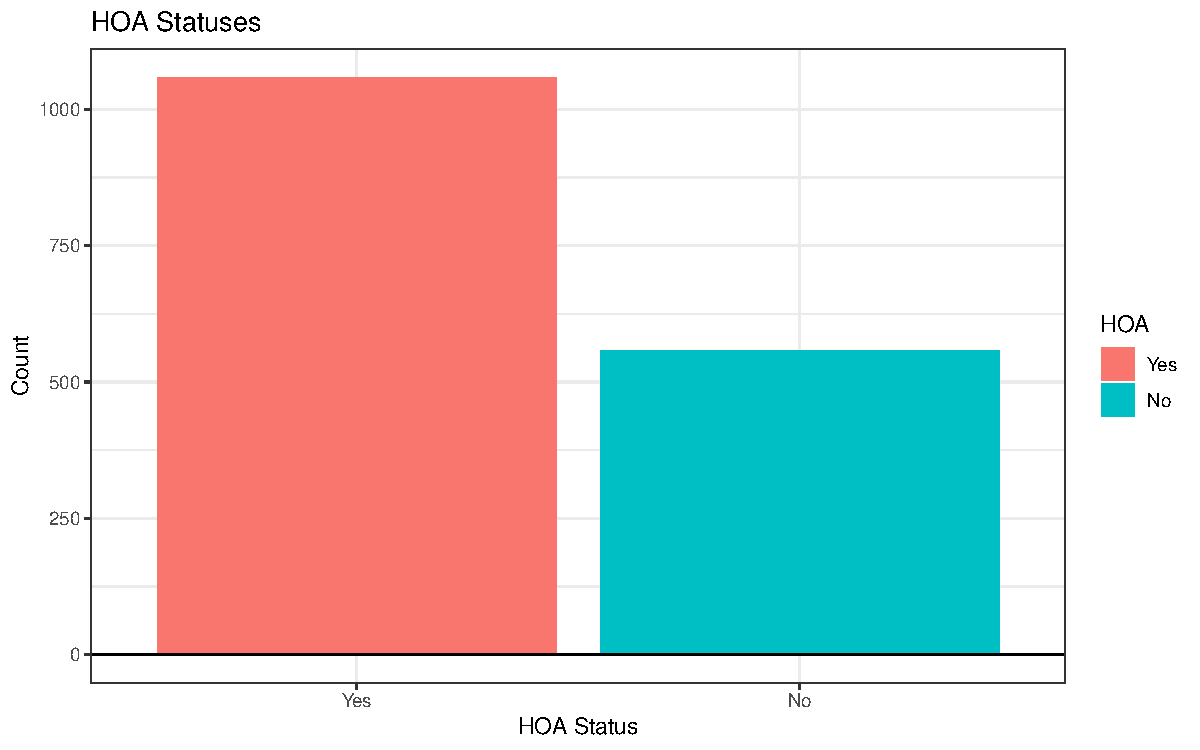
\includegraphics{exam22-008}
\begin{table}[h]
\begin{tabular}{|c|c|} \hline
HOA Status & Frequency \\ \hline
HOA        & 0.659176  \\ \hline
NoN HOA    & 0.340824 \\ \hline
\end{tabular}
\end{table}

There seems to be almost twice as many homes in our sample that are a part of an HOA as homes that are not a part of an HOA. To be precise, 65.91 percent of homes in our sample are HOA homes and 34.08 percent of homes in our sample are non HOA homes. 


We should also look at these numbers in reference to different factors and compare breakdowns with homes that are part of an HOA and those that are not.


The next graphs provide a side-by-side comparisons of households in HOAs and households not in HOAs, representing the relationships between these households' HOA statuses and multiple sustainability indicators. These graphs all utilize relative frequencies to compare proportionally between HOA households and non HOA households. As was illustrated by the graph above, over 60 percent of the households in the sample are in an HOA while about 30 percent of households in the sample are not in an HOA. This will be important as we begin to analyze the homes by different factors. 

\newpage
\textsc{\textbf{Recycling and HOA Statuses}}
\newline
\newline
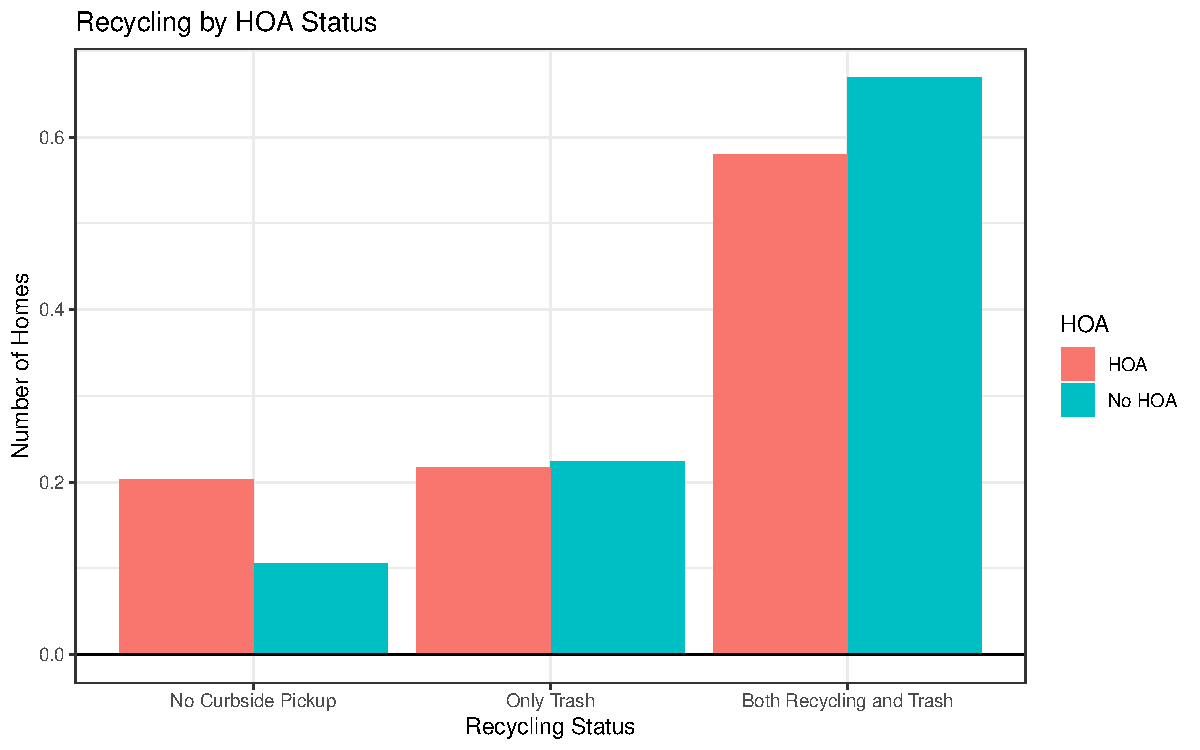
\includegraphics{exam22-009}

\begin{Schunk}
\begin{Sinput}
> #dat.HOA$HOA<-factor(dat.HOA$HOA, levels=c(1,2),labels = c("Yes", "No"))
> dat.HOA$Recycle<-factor(dat.HOA$Recycle, levels = c(0,1,2),
+                         labels = c("No Curbside Pickup",
+                         "Only Trash","Both Recycling and Trash"))
> prop.table(table(dat.HOA$Recycle, dat.HOA$HOA),margin=2)*100
\end{Sinput}
\begin{Soutput}
                                Yes       No
  No Curbside Pickup       20.30217 10.59246
  Only Trash               21.71860 22.44165
  Both Recycling and Trash 57.97923 66.96589
\end{Soutput}
\end{Schunk}

As we can see, regardless of HOA status homes the majority typically had both recycling and trash present. About 58 percent of HOA households and 67 percent of non HOA households had both trash and recycling pickup present. There were about the same proportion of homes that had only trash pickup for HOA and non HOA households (21.7 percent and 22.4 percent, respectively). About double the proportion of HOA households have no curbside pickup (20.3 percent) as non HOA households (10.6 percent). We see that there is a higher proportion of non HOA homes to HOA homes that have either trash pickup or both recycling and trash pick up rather than no curbside pickup. This suggests that non HOA homes may be better for the environment compared to HOA homes in regards to recycling and waste management.

We aim to quantify the relationship between recycling status and HOA status using the chi-squared test, a test that assesses the relationship between a categorical variable and k categories, which is also a nonparametric alternative to the Fisher test.

The null hypothesis is that the two categorical variables, recycling status and HOA status, are independent.
The alternative hypothesis is that the two categorical variables, recycling status and HOA status, are dependent. 

There are several assumptions we need to hold. 

The first is that the two variables are categorical, which is true.

The second is that the observations are independent. While this isn't necessarily true, as neighbors can affect each other's behavior, for our purposes we will assume this to be true. Each household is only reported once. 

The third is that the sample size is at least the number of cells in the table multiplied by 5. If there are 3 recycling statuses and 2 HOA statuses, so 6 cells total, 1616 is more than 5 times larger than 6 (30). 

We need to check our expected counts, or the number of observations that we would expect to see in a cell if the observations were truly independent (if the null hypothesis is true). We need to ensure 80\% of expected counts are greater than 5. This is calculated by multiplying the total of row i by the total of column j and dividing this quantity by n. We can do this for HOA and non HOA households. 

\begin{Schunk}
\begin{Sinput}
> rHOA<-table(dat.HOA$Recycle,dat.HOA$HOA)
> rHOA1<-addmargins(rHOA)
> rHOA1
\end{Sinput}
\begin{Soutput}
                            Yes   No  Sum
  No Curbside Pickup        215   59  274
  Only Trash                230  125  355
  Both Recycling and Trash  614  373  987
  Sum                      1059  557 1616
\end{Soutput}
\begin{Sinput}
> prop.table(rHOA)
\end{Sinput}
\begin{Soutput}
                                  Yes         No
  No Curbside Pickup       0.13304455 0.03650990
  Only Trash               0.14232673 0.07735149
  Both Recycling and Trash 0.37995050 0.23081683
\end{Soutput}
\end{Schunk}
(274 x 1059)/1616=179.56
\newline{(987 x 1059)/1616=646.80}
\newline{(355 x 1059)/1616=232.64}
\newline{(274 x 557)/1616=94.44}
\newline{(987 x 557)/1616=340.20}
\newline{(355 x 557)/1616=122.36}

As we can see, all expected counts are greater than 5.

Lastly, we need to confirm that none of the expected counts are less than one, which is true in these cases. 

We can now calculate test statistics for the chi-square tests. 
\begin{Schunk}
\begin{Sinput}
> chisq.test(x=dat.HOA$Recycle,y=dat.HOA$HOA)
\end{Sinput}
\begin{Soutput}
	Pearson's Chi-squared test

data:  dat.HOA$Recycle and dat.HOA$HOA
X-squared = 25.209, df = 2, p-value = 3.356e-06
\end{Soutput}
\end{Schunk}

As we can see for HOA households, the test statistic is 25.209 and the p-value is essentially zero, which is less than 0.05. We therefore can reject the null hypothesis and conclude that there is sufficient evidence to suggest that there is a relationship between recycling status and HOA status. This means that in terms of sustainability, we can use recycling status as a determinant for HOA.

\newpage
\textsc{\textbf{Lawn Care and HOA Statuses}}
\newline
\newline
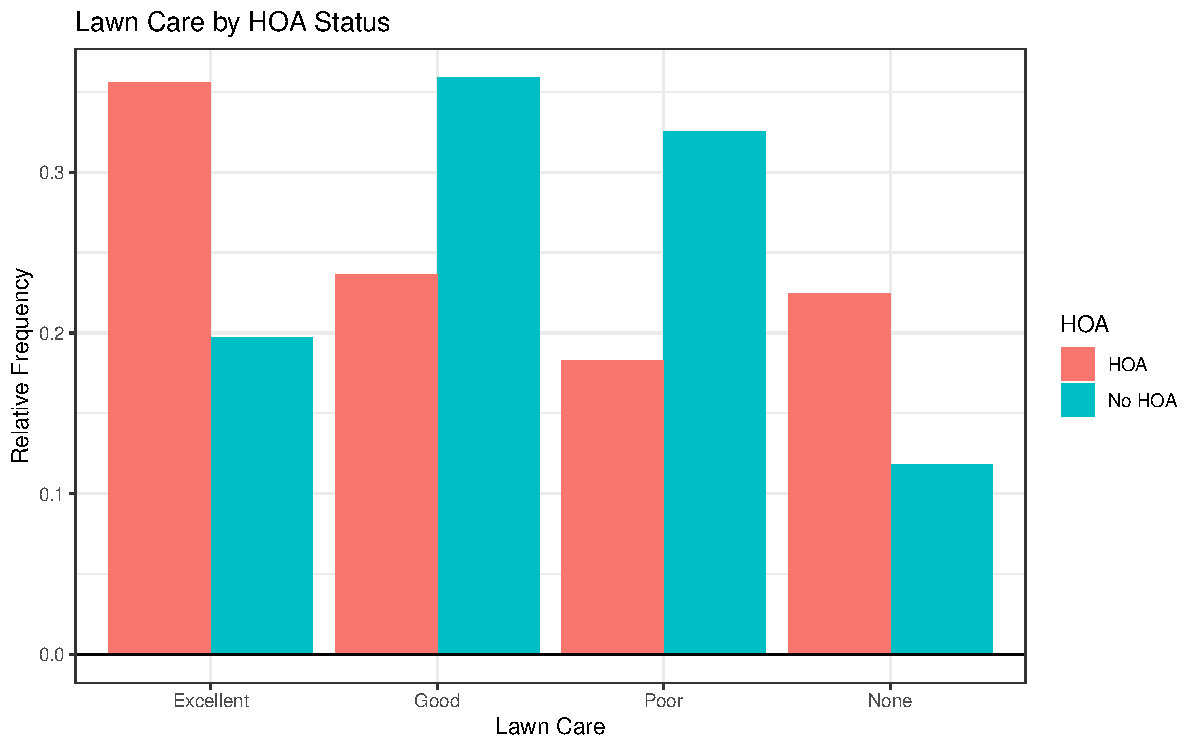
\includegraphics{exam22-013}

\begin{Schunk}
\begin{Sinput}
> dat.HOA$LawnCare<-factor(dat.HOA$LawnCare, levels = c(1,2,3,4),
+                         labels = c("Excellent",
+                         "Good",
+                         "Poor",
+                         "None"))
> prop.table(table(dat.HOA$LawnCare, dat.HOA$HOA),margin=2)*100
\end{Sinput}
\begin{Soutput}
                 Yes       No
  Excellent 35.59962 19.74865
  Good      23.60718 35.90664
  Poor      18.31917 32.49551
  None      22.47403 11.84919
\end{Soutput}
\end{Schunk}

As you can see from the charts above, households in HOAs had a higher percent of excellent lawn care (35.6 percent) than households without HOAs (19.7 percent). From this, we can infer that these households with HOAs typically use more chemical application than those without HOAs, which is worse for the environment. We also see that the highest percentage of homes not in an HOA have good (35.9 percent) or poor (32.5 percent) lawn care relative to homes in HOAs (23.7 percent and 18.4 percent, respectively). How much more damaging non HOA homes are compared to HOA homes in regards to lawn care is hard to say from the graph alone, but we can see from the table that more HOA households had excellent or good lawn care (about 59 percent) compared to non HOA households (about 56 percent). Again though, lawn care status alone may not be enough to determine if HOA households or non HOA households are better or worse for the environment. 

Again, now that we have a better picture of the data we can perform statistical analyses to determine whether or not lawn care differs significantly by HOA status. 

We aim to quantify the relationship between lawn care and HOA status using the chi-squared test.

The null hypothesis is that the two categorical variables, lawn care and HOA status, are independent.
The alternative hypothesis is that the two categorical variables, lawn care and HOA status, are dependent. 

There are several assumptions we need to hold. 

The first is that the two variables are categorical, which is true.

The second is that the observations are independent. While this isn't necessarily true, as neighbors can affect each other's behavior, for our purposes we will assume this to be true. Each household is only reported once. 

The third is that the sample size is at least the number of cells in the table multiplied by 5. If there are 4 lawn care statuses and 2 HOA statuses, so 8 cells total, 1616 is more than 5 times larger than 8 (40). 

We need to check our expected counts, or the number of observations that we would expect to see in a cell if the observations were truly independent (if the null hypothesis is true). We need to ensure 80\% of expected counts are greater than 5. This is calculated by multiplying the total of row i by the total of column j and dividing this quantity by n. We can do this for HOA and non HOA households. 

\begin{Schunk}
\begin{Sinput}
> lcHOA<-table(dat.HOA$LawnCare,dat.HOA$HOA)
> lcHOA1<-addmargins(lcHOA)
> lcHOA1
\end{Sinput}
\begin{Soutput}
             Yes   No  Sum
  Excellent  377  110  487
  Good       250  200  450
  Poor       194  181  375
  None       238   66  304
  Sum       1059  557 1616
\end{Soutput}
\begin{Sinput}
> prop.table(lcHOA)
\end{Sinput}
\begin{Soutput}
                   Yes         No
  Excellent 0.23329208 0.06806931
  Good      0.15470297 0.12376238
  Poor      0.12004950 0.11200495
  None      0.14727723 0.04084158
\end{Soutput}
\end{Schunk}
(487 x 1059)/1616=319.14
\newline{(450 x 1059)/1616=294.89}
\newline{(375 x 1059)/1616=245.75}
\newline{(304 x 1059)/1616=199.22}
\newline{(487 x 557)/1616=167.86}
\newline{(450 x 557)/1616=155.11}
\newline{(375 x 557)/1616=129.25}
\newline{(304 x 557)/1616=104.78}

As we can see, all expected counts are greater than 5.

Lastly, we need to confirm that none of the expected counts are less than one, which is true in these cases. 

We can now calculate test statistics for the chi-square tests. 
\begin{Schunk}
\begin{Sinput}
> chisq.test(x=dat.HOA$LawnCare,y=dat.HOA$HOA)
\end{Sinput}
\begin{Soutput}
	Pearson's Chi-squared test

data:  dat.HOA$LawnCare and dat.HOA$HOA
X-squared = 103.78, df = 3, p-value < 2.2e-16
\end{Soutput}
\end{Schunk}

As we can see for HOA households, the test statistic is 103.78 and the p-value is essentially zero, which is less than 0.05. We therefore can reject the null hypothesis and conclude that there is sufficient evidence to suggest that there is a relationship between lawn care status and HOA status. This is important when evaluating sustainbility factors and HOA status as we have found now that lawn care is now significantly related to HOA.

\newpage
\textsc{\textbf{Trees in Yard and HOA Statuses}}
\newline
\newline
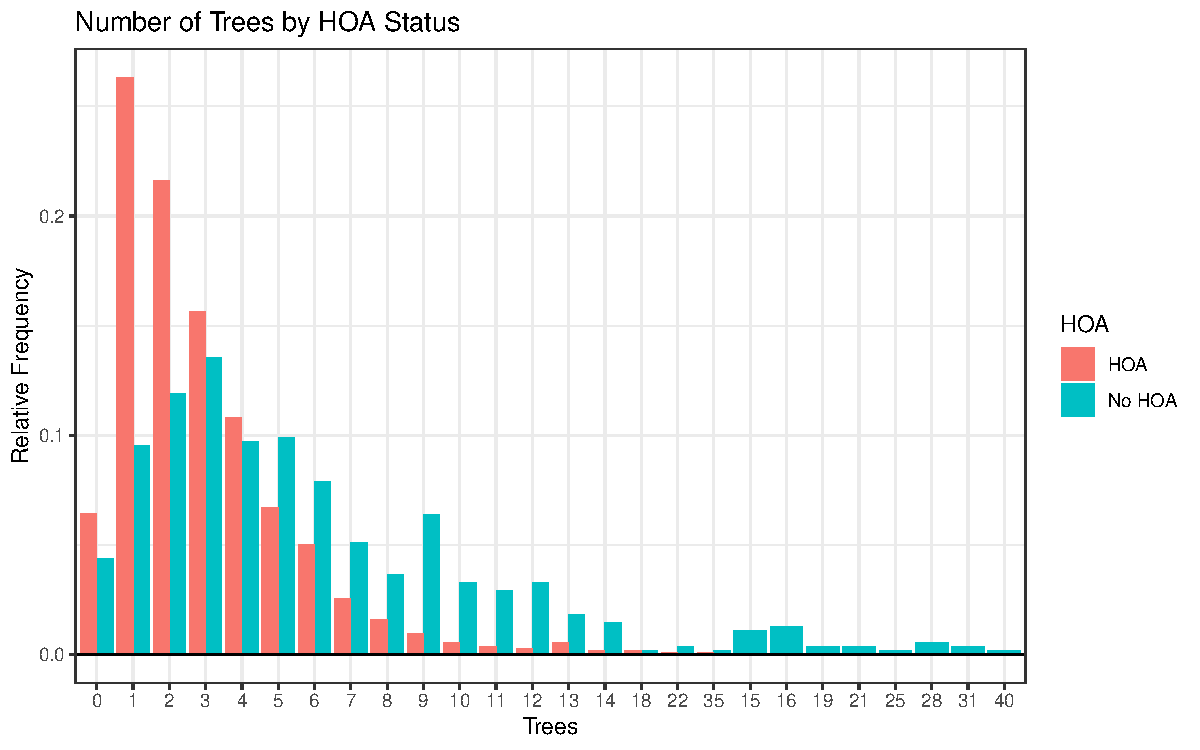
\includegraphics{exam22-017}

\begin{Schunk}
\begin{Sinput}
> prop.table(table(dat.HOA$Trees, dat.HOA$HOA),margin=2)*100
\end{Sinput}
\begin{Soutput}
             Yes          No
  0   6.43939394  4.39560440
  1  26.32575758  9.52380952
  2  21.59090909 11.90476190
  3  15.62500000 13.55311355
  4  10.79545455  9.70695971
  5   6.72348485  9.89010989
  6   5.01893939  7.87545788
  7   2.55681818  5.12820513
  8   1.60984848  3.66300366
  9   0.94696970  6.41025641
  10  0.56818182  3.29670330
  11  0.37878788  2.93040293
  12  0.28409091  3.29670330
  13  0.56818182  1.83150183
  14  0.18939394  1.46520147
  15  0.00000000  1.09890110
  16  0.00000000  1.28205128
  18  0.18939394  0.18315018
  19  0.00000000  0.36630037
  21  0.00000000  0.36630037
  22  0.09469697  0.36630037
  25  0.00000000  0.18315018
  28  0.00000000  0.54945055
  31  0.00000000  0.36630037
  35  0.09469697  0.18315018
  40  0.00000000  0.18315018
\end{Soutput}
\begin{Sinput}
> summary(dat.HOA$Trees)
\end{Sinput}
\begin{Soutput}
   Min. 1st Qu.  Median    Mean 3rd Qu.    Max.    NA's 
  0.000   1.000   3.000   3.952   5.000  40.000      14 
\end{Soutput}
\end{Schunk}

This figure illustrates the comparison between HOA homes and non HOA homes and the number of trees they have in their yard. It is important to note though that while most households in HOAs typically tend to have between 0 and 10 trees, it seems that households not in HOAs typically tend to have between 0 and 15 trees. In fact, about 62 percent of HOA homes have between 1 and 3 trees, where about half the proportion of non HOA homes (about 33 percent) have between 1 and 3 trees. The distribution of non HOA homes is less right skewed than the distribution of HOA homes, meaning a larger proportion of non HOA homes have more trees than HOA homes. From this, we can hypothesize that non HOA homes are more sustainable than HOA homes in the sense that non HOA homes have more trees planted than HOA homes, which is better for the environment.

We can now perform a hypothesis test to determine numerically if the number of trees in a yard varies across treatments of HOA and non HOA homes. When we see the sumarized data, we see that there are 14 \textit{NA} values, as was known to us from the description of the data. We can therefore utilize our subset of data with the 14 \textit{NA} values removed so that we can perform numerical analysis. Before deciding what test to use, we must first test for normality for the quantitative data.
\newline
\begin{Schunk}
\begin{Soutput}
<ggproto object: Class FacetGrid, Facet, gg>
    compute_layout: function
    draw_back: function
    draw_front: function
    draw_labels: function
    draw_panels: function
    finish_data: function
    init_scales: function
    map_data: function
    params: list
    setup_data: function
    setup_params: function
    shrink: TRUE
    train_scales: function
    vars: function
    super:  <ggproto object: Class FacetGrid, Facet, gg>
\end{Soutput}
\end{Schunk}
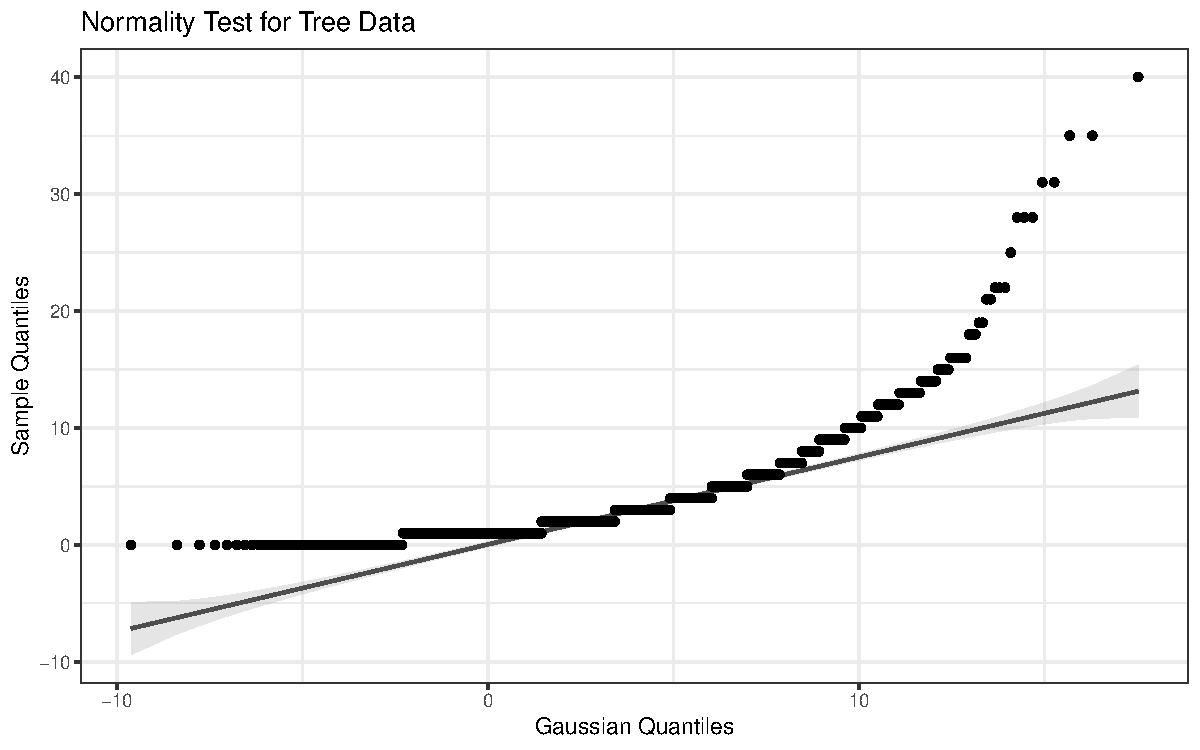
\includegraphics{exam22-019}

As we can see from the plots\citep{qqplotr}, the data is not normally distributed, but follows a parabolic shape. Therefore, for robustness, we perform a Mood's Median Test\citep{RVAideMemoire}. We want to generally identify if there is a difference across treatments, where the treatment is HOA versus non HOA. We look at these treatments specifically in the context of number of trees. We assume a representative sample. While these observations are not necessarily independent, since neighbors may base their recycling choices off of each other, for the sake of our study we will assume them to be so.

Our null hypothesis is that there is no significant difference between HOA and non HOA households with regards to recycling statuses; the population medians are all equal. Our alternative hypothesis is that there is a significant difference between HOA and non HOA households with regard to recycling statuses; at least one of the population medians is different. Since the plots of the data do not point towards normality, we will use a Mood's Median Test which is a nonparametric alternative to the ANOVA.

\begin{Schunk}
\begin{Sinput}
> #moods median test to determine if there are any significant differences
> #across treatments
> library(RVAideMemoire)
> mood.medtest(Trees~HOA,data=dat.HOA1)
\end{Sinput}
\begin{Soutput}
	Mood's median test

data:  Trees by HOA
X-squared = 138.67, df = 1, p-value < 2.2e-16
\end{Soutput}
\end{Schunk}

The Mood's median test is a chi-squared test that tests for differences across medians for quantitative data. Our chi-squared variable is 138.67 and our p-value is essentially zero. Since our p value is less than 0.05, we reject the null. This means that there is a significant relationship between HOA status and number of trees in the yard of a household.

We can perform a post-hoc test to adjust the p-value according to the number of groups. For Mood's Median Tests, we perform a Pairwise Median Test. 

\begin{Schunk}
\begin{Sinput}
> #pairwise to find particular difference
> library(rcompanion)
> PTBH<-pairwiseMedianTest(Trees~HOA,
+                        data   = dat.HOA1,
+                        method = "BH")
\end{Sinput}
\end{Schunk}

\begin{Schunk}
\begin{Sinput}
> cldList(p.adjust ~ Comparison,
+         data = PTBH,
+         threshold = 0.05)
\end{Sinput}
\begin{Soutput}
  Group Letter MonoLetter
1     1      a         a 
2     2      b          b
\end{Soutput}
\end{Schunk}

I utilize the Benjamini Hochberg approach \citep{rcompanion} to adjusting p-values because having a Type I error is not catatstrophic in this case. We see that with the p-value adjustemnt, HOA and non HOA households are still significantly different from each other in terms of number of trees in a yard.

\newpage
\textsc{\textbf{Garden and HOA Statuses}}
\newline
\newline
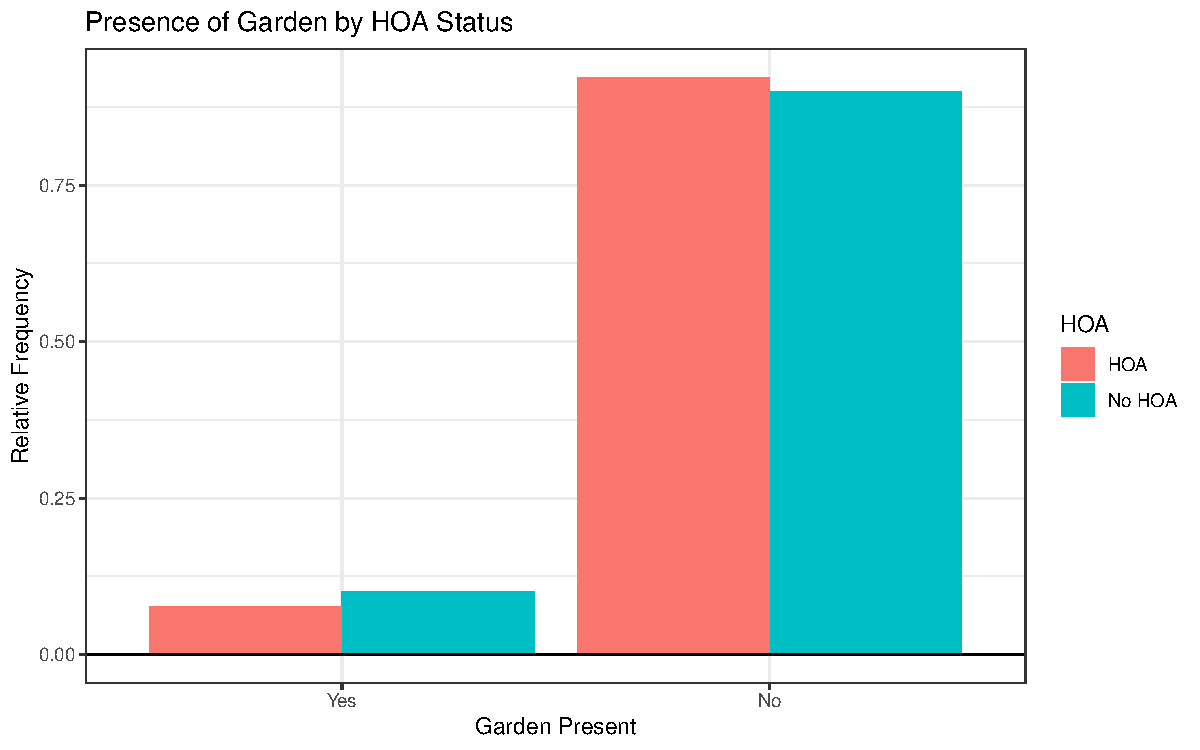
\includegraphics{exam22-023}

\begin{Schunk}
\begin{Sinput}
> dat.HOA$Garden<-factor(dat.HOA$Garden, levels = c(1,2),
+                         labels = c("Yes", "No"))
> prop.table(table(dat.HOA$Garden, dat.HOA$HOA),margin=2)*100
\end{Sinput}
\begin{Soutput}
            Yes        No
  Yes  7.743154 10.053860
  No  92.256846 89.946140
\end{Soutput}
\end{Schunk}

Households in and not in HOAs tend to follow a similar pattern when it comes to gardens. Both tend to not have gardens present in the front or back of their homes. 92.2 percent of HOA homes and 89.9 percent of non HOA homes did not have gardens in the yards. Therefore, in terms of garden status, HOA homes and non HOA homes have a similar, positive effect on the environment by not having gardens. This is under the assumption that it is possible to overplant, which is bad for the environment. However, it is important to note that this is a judgement call as some gardens may benefit the environment, but we have no way to know from just viewing pictures.

We can perform a hypothesis test to determine whether or not there is a statistically significant difference between HOA homes and non HOA homes and across Garden status. 

We aim to quantify the relationship between garden status and HOA status using the chi-squared test.

The null hypothesis is that the two categorical variables, garden status and HOA status, are independent.
The alternative hypothesis is that the two categorical variables, garden status and HOA status, are dependent. 

There are several assumptions we need to hold. 

The first is that the two variables are categorical, which is true.

The second is that the observations are independent. While this isn't necessarily true, as neighbors can affect each other's behavior, for our purposes we will assume this to be true. Each household is only reported once. 

The third is that the sample size is at least the number of cells in the table multiplied by 5. If there are 2 garden statuses and 2 HOA statuses, so 4 cells total, 1616 is more than 5 times larger than 4 (20). 

We need to check our expected counts, or the number of observations that we would expect to see in a cell if the observations were truly independent (if the null hypothesis is true). We need to ensure 80\% of expected counts are greater than 5. This is calculated by multiplying the total of row i by the total of column j and dividing this quantity by n. We can do this for HOA and non HOA households. 

\begin{Schunk}
\begin{Sinput}
> gHOA<-table(dat.HOA$Garden,dat.HOA$HOA)
> gHOA1<-addmargins(gHOA)
> gHOA1
\end{Sinput}
\begin{Soutput}
       Yes   No  Sum
  Yes   82   56  138
  No   977  501 1478
  Sum 1059  557 1616
\end{Soutput}
\begin{Sinput}
> prop.table(gHOA)
\end{Sinput}
\begin{Soutput}
             Yes         No
  Yes 0.05074257 0.03465347
  No  0.60457921 0.31002475
\end{Soutput}
\end{Schunk}
(138 x 1059)/1616=90.43
\newline{(1478 x 1059)/1616=968.57}
\newline{(138 x 557)/1616=47.57}
\newline{(1478 x 557)/1616=509.43}

As we can see, all expected counts are greater than 5.

Lastly, we need to confirm that none of the expected counts are less than one, which is true in these cases. 

We can now calculate test statistics for the chi-square tests. 
\begin{Schunk}
\begin{Sinput}
> chisq.test(x=dat.HOA$Garden,y=dat.HOA$HOA)
\end{Sinput}
\begin{Soutput}
	Pearson's Chi-squared test with Yates' continuity correction

data:  dat.HOA$Garden and dat.HOA$HOA
X-squared = 2.2082, df = 1, p-value = 0.1373
\end{Soutput}
\end{Schunk}

As we can see for HOA households, the test statistic is 2.2082 and the p-value is 0.1373, which is greater than 0.05. We therefore fail to reject the null hypothesis and conclude that there is not sufficient evidence to suggest that there is a relationship between garden status and HOA status. This means that since garden status is not significantly different across HOA statuses, we may consider not utilizing this variable in our multi-indicator analyses.

\noindent\rule{16cm}{0.4pt}
\newline
After examining sustainability factors at the household level, we can see that recycling status, lawn care, and number of trees in a yard are all significantly different across HOA statuses. Garden status is not significantly different across HOA and non HOA statuses. This is due to the fact that HOA and non HOA homes followed the same pattern of garden status, as was seen in our plot. 

It is important to also recognize some drawbacks of the data we have while interpretting our initial results and before we continue on with multi-indicator analyses. The lawn care variable should be interpretted cautiously. Without knowing how many/much chemicals were used for the different lawn statuses of "excellent", "good", and "poor", it is hard to determine the environmental effects of homes in each category. Garden status is hard to interpret, again because it is not specified what the criteria was of a garden, whether fertilizer was used or not, if pesticides were used or not, etc. It is hard to tell if trees were planted or grew from the ground naturally and how these affect ecosystems. For recycling, if there is no curbside pickup, we don't know how the garbage and recycling are dealt with. 

Now that we've seen the general count of observations with and without HOA, we can begin to examine multi-indicator sustainability analyses.

%Before doing further analyses with the data, we can split up neighborhoods by their HOA status.

%Neighborhoods with HOAs are: Brownstone Crossing, Edgewood at Paris, Glastonbury Village, Half Mile Lake, Northcliff, Patridge Ridge

%Neighborhoods without HOAs are: Buxton, Croftstone Acres, Fox Springs, Liberty Park, Timberlake, Windermere

We will continue our multi-indicator sustainbility analyses of the households using our 3 statistically significant variables: Recycling Status, Lawn Care, and Trees.

\newpage
\textsc{\textbf{Relationship between Lawn Care and Recycling}}
\newline
\newline
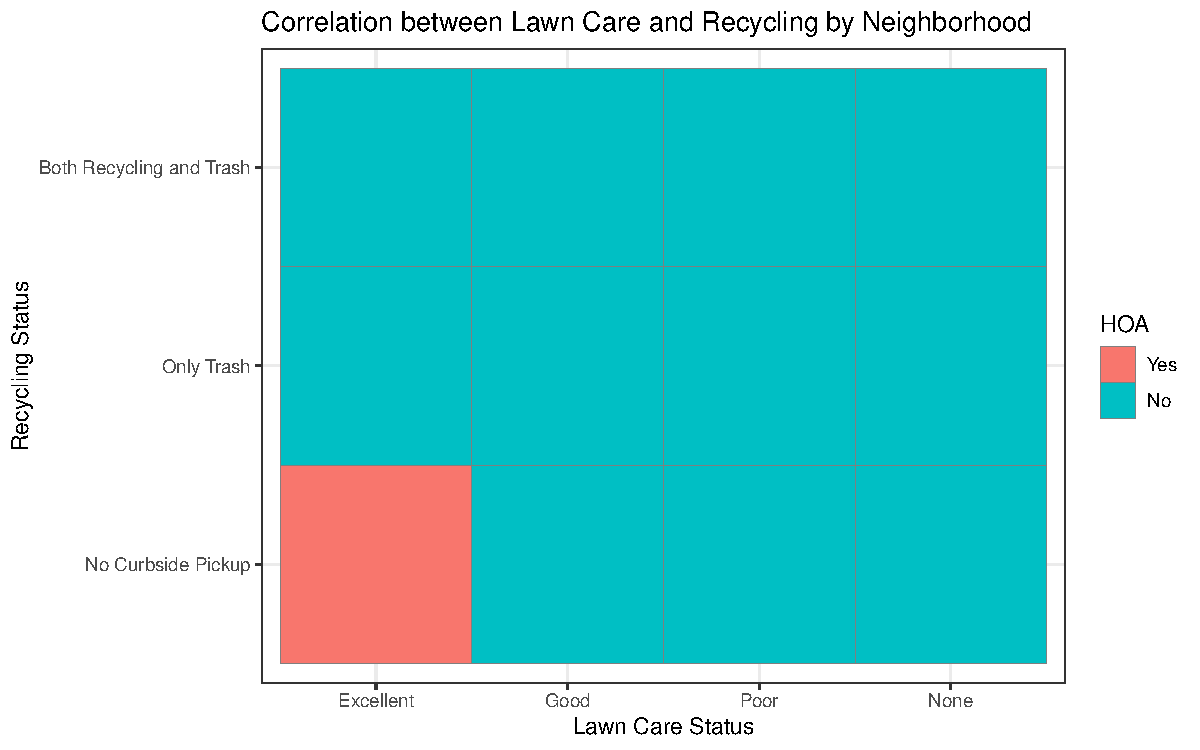
\includegraphics{exam22-027}

As we can see from the tile plot above, HOA homes are more associated with excellent lawn care and no curbside pickup for recycling, while non HOA homes are more associated with all other categories. This points us to believe that HOA homes are less sustainable than non HOA homes because they are associated with unsustainable practices while non HOA homes are not. We can look at tables of the data get more insight. 
\begin{Schunk}
\begin{Soutput}
         1    2    3    4  Sum
  0     83   53   33   46  215
  1     56   48   55   71  230
  2    238  149  106  121  614
  Sum  377  250  194  238 1059
\end{Soutput}
\begin{Soutput}
             1          2          3          4
  0 0.07837583 0.05004721 0.03116147 0.04343720
  1 0.05288008 0.04532578 0.05193579 0.06704438
  2 0.22474032 0.14069877 0.10009443 0.11425873
\end{Soutput}
\begin{Soutput}
        1   2   3   4 Sum
  0    12  19  18  10  59
  1    16  52  44  13 125
  2    82 129 119  43 373
  Sum 110 200 181  66 557
\end{Soutput}
\begin{Soutput}
             1          2          3          4
  0 0.02154399 0.03411131 0.03231598 0.01795332
  1 0.02872531 0.09335727 0.07899461 0.02333932
  2 0.14721724 0.23159785 0.21364452 0.07719928
\end{Soutput}
\end{Schunk}

\begin{center} Recycling Status by Lawn Care Status for HOA \end{center}
\begin{table}[H]
\begin{tabular}{|c|c|c|c|c|} \hline
                           & None       & Poor       & Good       & Excellent  \\ \hline
No Trash Pickup            & 0.07859848 & 0.05018939 & 0.03125000 & 0.04356061 \\ \hline
Trash and Recycling Pickup & 0.22537879 & 0.14109848 & 0.10037879 & 0.11268939 \\ \hline
Trash Pickup Only          & 0.05208333 & 0.04545455 & 0.05208333 & 0.06723485 \\ \hline
\end{tabular}
\end{table}

\begin{center} Recycling Status by Lawn Care Status for non HOA \end{center}
\begin{table}[H]
\begin{tabular}{|c|c|c|c|c|} \hline
                           & None       & Poor       & Good       & Excellent  \\ \hline
No Trash Pickup            & 0.02197802 & 0.03479853 & 0.03296703 & 0.01831502 \\ \hline
Trash and Recycling Pickup & 0.14835165 & 0.23443223 & 0.21428571 & 0.06776557 \\ \hline
Trash Pickup Only          & 0.02747253 & 0.09523810 & 0.08058608 & 0.02380952 \\ \hline
\end{tabular}
\end{table}

As we can see from the tables, about 60 percent of non HOA households have both Trash and Recycling Pickup and none, poor, or good lawn care. About 46 percent of HOA households have both Trash and Recycling Pickup and none, poor, or good lawn care. This is important because it shows that non HOA neighborhoods have a larger proportion of their homes following good sustainability trends compared to HOA neighborhoods. 

We can perform an association test to see if recycling and lawn care are associated by HOA. To do so, we can perform a chi-square independence test.

We can test whether observed dependence of recycling status and lawn care by HOA is due to random chance or not. 

The null hypothesis is that the two categorical variables, recycling status and lawn care, are independent.
The alternative hypothesis is that the two categorical variables, recycling status and lawn care, are dependent. 

There are several assumptions we need to hold for HOA and non HOA households. 

The first is that the two variables are categorical, which is true.

The second is that the observations are independent. While this isn't necessarily true, as neighbors can affect each other's behavior, for our purposes we will assume this to be true. Each household is only reported once. 

The third is that the sample size is at least the number of cells in the table multiplied by 5. If there are 3 recycling statuses and 4 lawn care statuses, so 12 cells total, 1616 is more than 5 times larger than 12(60). 

We need to check our expected counts, or the number of observations that we would expect to see in a cell if the observations were truly independent (if the null hypothesis is true). We need to ensure 80\% of expected counts are greater than 5. This is calculated by multiplying the total of row i by the total of column j and dividing this quantity by n. We can do this for HOA and non HOA households. 
\newline{HOA Households}
\newline{(215 x 377)/1616=50.16}
\newline{(614 x 377)/1616=143.24}
\newline{(230 x 377)/1616=53.66}
\newline{(215 x 250)/1616=33.26}
\newline{(614 x 250)/1616=94.99}
\newline{(230 x 250)/1616=35.58}
\newline{(215 x 194)/1616=25.81}
\newline{(614 x 194)/1616=73.71}
\newline{(230 x 194)/1616=27.61}
\newline{(215 x 238)/1616=31.66}
\newline{(614 x 238)/1616=90.42}
\newline{(230 x 238)/1616=33.87}
\newline
\newline{Non HOA Households}
\newline{(59 X 110)/1616=4.02}
\newline{(373 X 110)/1616=25.39}
\newline{(125 X 110)/1616=8.51}
\newline{(59 X 200)/1616=7.30}
\newline{(373 X 200)/1616=46.16}
\newline{(125 X 200)/1616=15.47}
\newline{(59 X 181)/1616=6.61}
\newline{(373 X 181)/1616=41.78}
\newline{(125 X 181)/1616=14.00}
\newline{(59 X 66)/1616=2.41}
\newline{(373 X 66)/1616=15.23}
\newline{(125 X 66)/1616=5.11}

As we can see, all expected counts are greater than 5 for the HOA sample and 10 out of 12 cells for the non HOA sample or about 83\% of cells are greater than 5.

Lastly, we need to confirm that none of the expected counts are less than one, which is true in these cases. 

We can now calculate test statistics for the chi-square tests. 
\begin{Schunk}
\begin{Sinput}
> #HOA homes
> chisq.test(x=dat.HOA.y$Recycle,y=dat.HOA.y$LawnCare)
\end{Sinput}
\begin{Soutput}
	Pearson's Chi-squared test

data:  dat.HOA.y$Recycle and dat.HOA.y$LawnCare
X-squared = 26.147, df = 6, p-value = 0.000209
\end{Soutput}
\begin{Sinput}
> #nonHOA homes
> chisq.test(x=dat.HOA.n$Recycle,y=dat.HOA.n$LawnCare)
\end{Sinput}
\begin{Soutput}
	Pearson's Chi-squared test

data:  dat.HOA.n$Recycle and dat.HOA.n$LawnCare
X-squared = 7.488, df = 6, p-value = 0.2781
\end{Soutput}
\end{Schunk}

As we can see for HOA households, the test statistic is 26.147 and the p-value is 0.0002, which is close to zero. We therefore can reject the null hypothesis and conclude that for HOA households, there is sufficient evidence to suggest that there is a relationship between recycling status and lawn care. This is important since both of these variables are related to HOA status. Comparing with the figure, we see that HOA observations are specifically concentrated with no curbside pickup and excellent lawn care, pointing to the fact that HOAs are not sustainable.

For non HOA households, the test statistic is 7.488 and the p-value is 0.2781, which is greater than 0.05. We therefore fail to reject the null hypothesis and conclude that for non HOA households, there is not sufficient evidence to suggest that there is a relationship between recycling status and lawn care. This suggests less consistency with sustainability factors for non HOA households.

\newpage
\textsc{\textbf{Relationship between Trees and Recycling}}
\newline
\newline
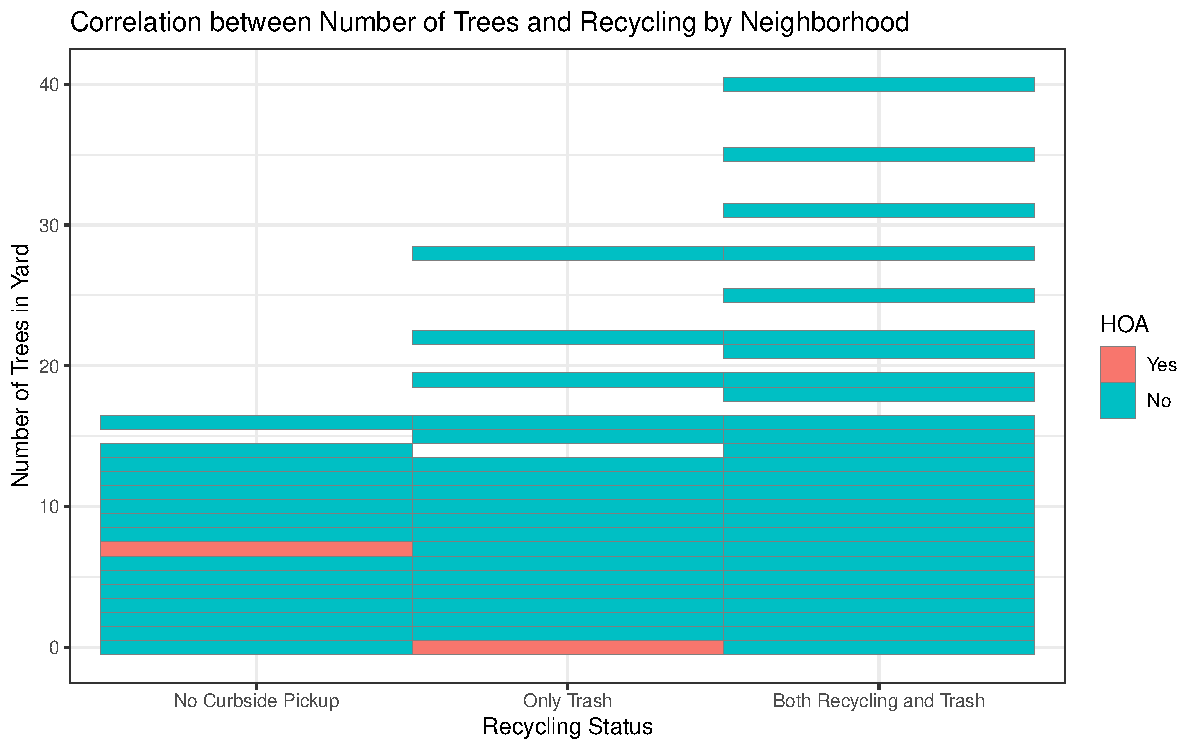
\includegraphics{exam22-030}

This graph illustrates that recycling and trash pickup is correlated with more trees for non HOA neighborhoods; non HOA neighborhoods have more trees generally. From this graph, we can posit that non HOA neighborhoods may be more sustainable than HOA neighborhoods because they have greater concentrations of numbers of trees and instances of recycling and trash pickup or trash pickup only. HOA neighborhoods seem to only have associations with only trash pickup and no trees, or no curbside pickup and 7 trees.

We can perform an association test to see if there is correlation between trees and recycling status by HOA. First, we must test for normality since we are dealing with quantitative data.  
\newline
\begin{Schunk}
\begin{Soutput}
<ggproto object: Class FacetGrid, Facet, gg>
    compute_layout: function
    draw_back: function
    draw_front: function
    draw_labels: function
    draw_panels: function
    finish_data: function
    init_scales: function
    map_data: function
    params: list
    setup_data: function
    setup_params: function
    shrink: TRUE
    train_scales: function
    vars: function
    super:  <ggproto object: Class FacetGrid, Facet, gg>
\end{Soutput}
\end{Schunk}
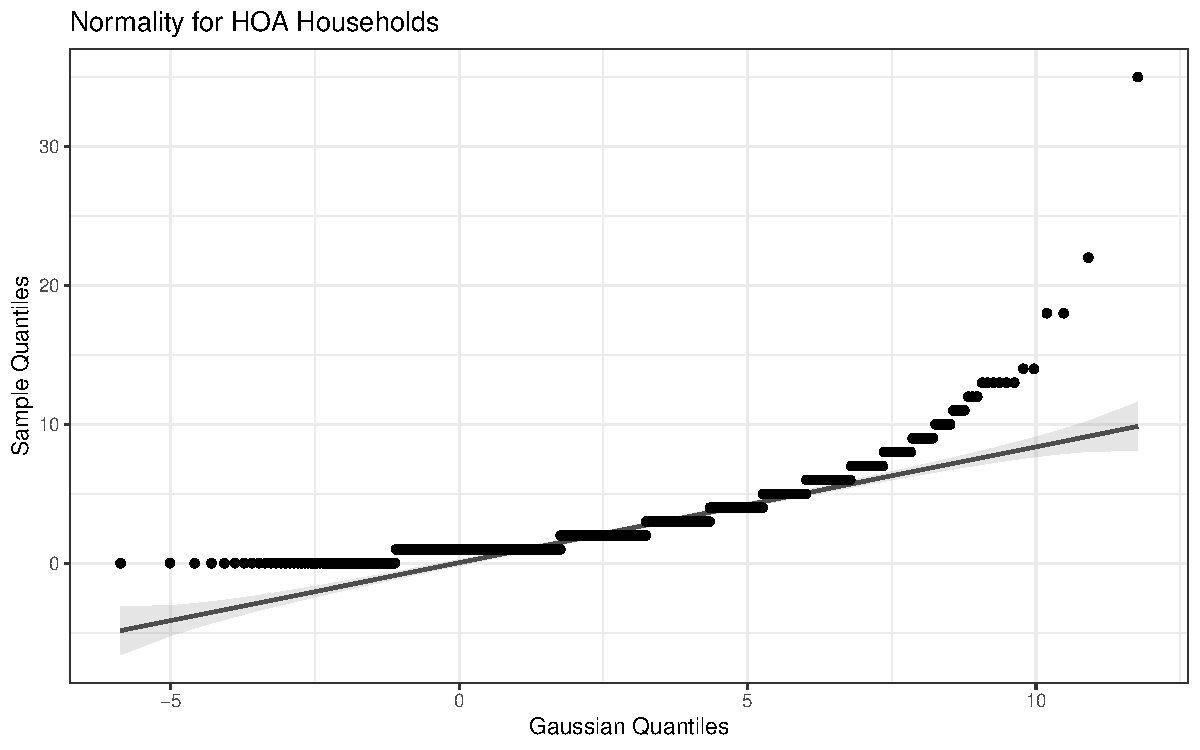
\includegraphics{exam22-031}

\begin{Schunk}
\begin{Soutput}
<ggproto object: Class FacetGrid, Facet, gg>
    compute_layout: function
    draw_back: function
    draw_front: function
    draw_labels: function
    draw_panels: function
    finish_data: function
    init_scales: function
    map_data: function
    params: list
    setup_data: function
    setup_params: function
    shrink: TRUE
    train_scales: function
    vars: function
    super:  <ggproto object: Class FacetGrid, Facet, gg>
\end{Soutput}
\end{Schunk}
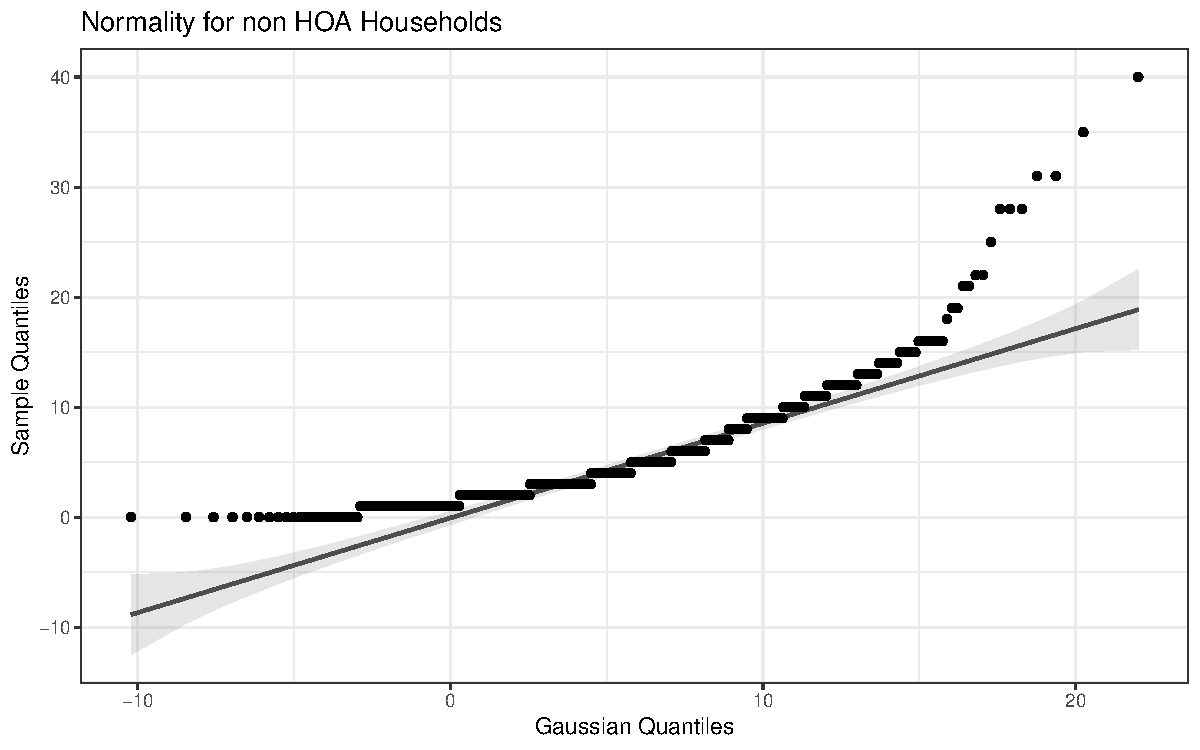
\includegraphics{exam22-032}

As we can see from the plots\citep{qqplotr}, the data is not normally distributed for HOA or non HOA homes, but follows a parabolic shape. Therefore, for robustness, we perform a Mood's Median Test\citep{RVAideMemoire}. We want to generally identify if there is a relationship between recycling and trees by HOA status. We assume representative samples. While these observations are not necessarily independent, since neighbors may base their recycling choices off of each other, for the sake of our study we will assume them to be so.

We run two tests simultaneously: one for HOA homes and one for non HOA homes.
Our hypotheses for the HOA homes is as follows. Our null hypothesis is that the population median of trees are equal for all recycling statuses. Our alternative hypothesis is that at least one of the population medians of trees is different for recycling statuses. Since the plots of the data do not point towards normality, we will use a Mood's Median Test which is a nonparametric alternative to the ANOVA.

Our hypotheses for the non HOA homes is as follows. Our null hypothesis is that the population median of trees are equal for all recycling statuses. Our alternative hypothesis is that at least one of the population medians of trees is different for recycling statuses. Since the plots of the data do not point towards normality, we will use a Mood's Median Test which is a nonparametric alternative to the ANOVA.

\begin{Schunk}
\begin{Sinput}
> #moods median test to determine if there are any significant differences
> #across treatments
> mood.medtest(Trees~Recycle,data=dat.HOA.notree.y)
\end{Sinput}
\begin{Soutput}
	Mood's median test

data:  Trees by Recycle
X-squared = 49.625, df = 2, p-value = 1.676e-11
\end{Soutput}
\begin{Sinput}
> mood.medtest(Trees~Recycle,data=dat.HOA.notree.n)
\end{Sinput}
\begin{Soutput}
	Mood's median test

data:  Trees by Recycle
X-squared = 5.3359, df = 2, p-value = 0.06939
\end{Soutput}
\end{Schunk}

The Mood's median test is a chi-squared test that tests for differences across medians. 

For HOA households, our chi-squared variable is 49.625 and our p-value is essentially zero, which is less than 0.05. Since our p value is less than 0.05, we reject the null. There is a significant difference of median trees across recycling statuses for HOA households. These lowers values of HOA homes then that we see in the plot are significant because they indicate that only trash recycling status and no trees are related. This again points us to believe that HOA homes are not sustainable because they are related to not recycling. 

For non HOA households, our chi-squared variable is 5.3359 and our p-value is 0.06939, which is greater than 0.05. Therefore, we fail to reject the null. There is not a significant difference of median trees across recycling statuses for non HOA households. 

\newpage
\textsc{\textbf{Relationship between Trees and Lawn Care}}
\newline
\newline
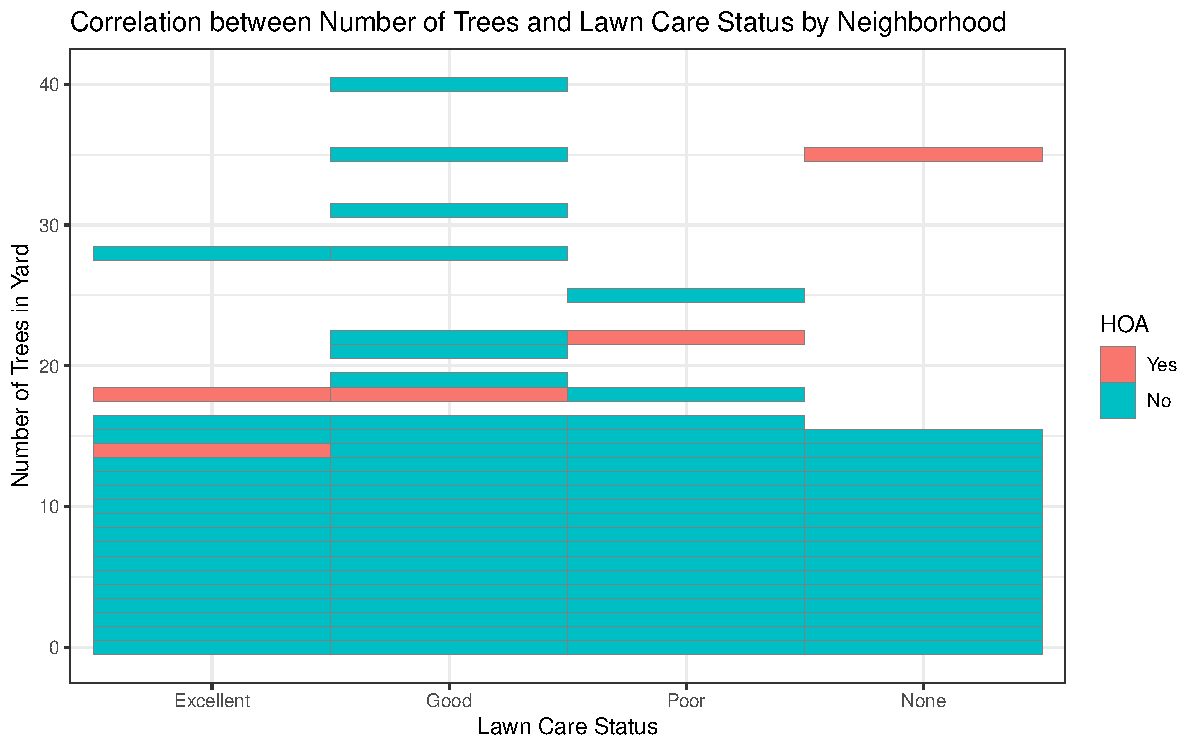
\includegraphics{exam22-034}

The graph above illustrates that non HOA neighborhoods could be more sustainable than HOA neighborhoods because non HOA homes are more likely to have more trees and less lawn care compared to HOA neighborhoods. As we can see, the two kinds of neighborhoods follow different patterns. Non HOA neighborhoods follow a right skew pattern, where most observations have a lot of trees and little lawn care and then decrease the amount of trees they have as they increase their lawn care. HOA neighborhoods follow an increasing exponential pattern where none and poor lawn care statuses have fewer trees and as lawn care improves, the amount of trees seen on the property increases.

We can examine this relationship further by performing an association test. 

We can perform an association test to see if there is correlation between trees and lawn care status by HOA. First, we must test for normality. 
\newline
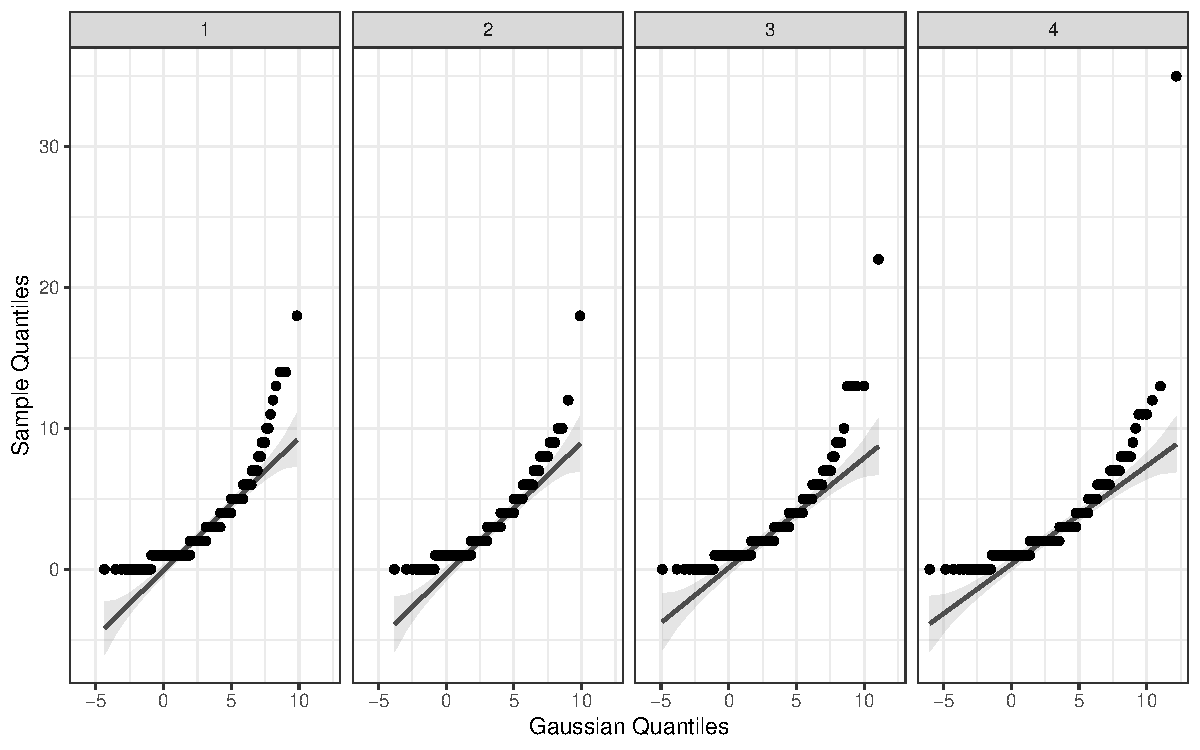
\includegraphics{exam22-035}

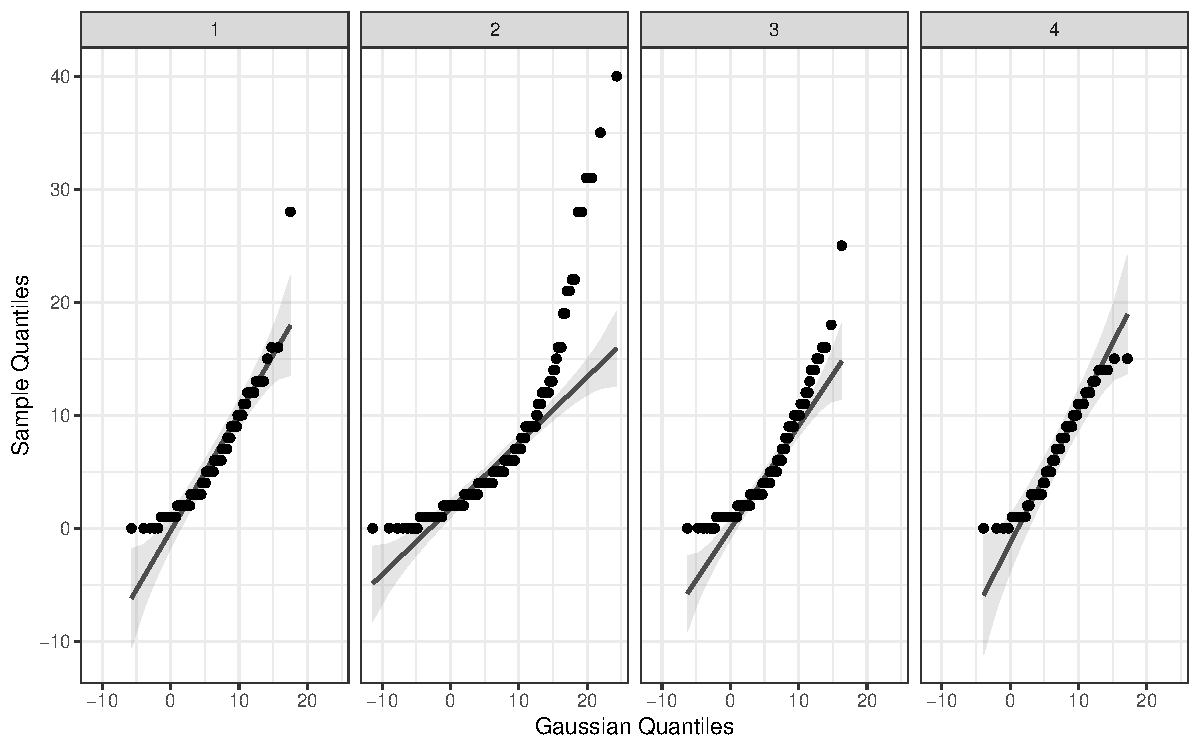
\includegraphics{exam22-036}

As we can see from the plots\citep{qqplotr}, the data is not normally distributed for HOA or non HOA homes, but follows a parabolic shape. Therefore, for robustness, we perform a Mood's Median Test\citep{RVAideMemoire}. We want to generally identify if there is a relationship between lawn care and trees by HOA status. We assume representative samples. While these observations are not necessarily independent, since neighbors may base their recycling choices off of each other, for the sake of our study we will assume them to be so.

We run two tests simultaneously: one for HOA homes and one for non HOA homes.
Our hypotheses for the HOA homes is as follows. Our null hypothesis is that the population median of trees are equal for all lawn care statuses. Our alternative hypothesis is that at least one of the population medians of trees is different for all lawn care statuses. Since the plots of the data do not point towards normality, we will use a Mood's Median Test which is a nonparametric alternative to the ANOVA.

Our hypotheses for the non HOA homes is as follows. Our null hypothesis is that the population median of trees are equal for all lawn care statuses. Our alternative hypothesis is that at least one of the population medians of trees is different for lawn care statuses. Since the plots of the data do not point towards normality, we will use a Mood's Median Test which is a nonparametric alternative to the ANOVA.

\begin{Schunk}
\begin{Sinput}
> #moods median test to determine if there are any significant differences
> #across treatments
> mood.medtest(Trees~LawnCare,data=dat.HOA.notree.y)
\end{Sinput}
\begin{Soutput}
	Mood's median test

data:  Trees by LawnCare
X-squared = 2.7752, df = 3, p-value = 0.4276
\end{Soutput}
\begin{Sinput}
> mood.medtest(Trees~LawnCare,data=dat.HOA.notree.n)
\end{Sinput}
\begin{Soutput}
	Mood's median test

data:  Trees by LawnCare
X-squared = 10.897, df = 3, p-value = 0.01229
\end{Soutput}
\end{Schunk}

For HOA households, our chi-squared variable is 2.7752 and our p-value is 0.4276. Since our p value is greater than 0.05, we fail to reject the null. There is not a significant median difference of trees in a yard by lawn care status for HOA homes. 

For non HOA households, our chi-squared variable is 10.897 and our p-value is 0.01229, which is less than 0.05. Therefore, reject the null. There is a significant difference in medians of trees in a yard by lawn care status for non HOA homes. 

We can perform a post-hoc test to adjust the p-value according to the number of groups. For Mood's Median Tests, we perform a Pairwise Median Test. 

\begin{Schunk}
\begin{Sinput}
> #pairwise to find particular difference
> library(rcompanion)
> PTBH<-pairwiseMedianTest(Trees~LawnCare,
+                        data   = dat.HOA.notree.n,
+                        method = "BH")
\end{Sinput}
\end{Schunk}

\begin{Schunk}
\begin{Sinput}
> cldList(p.adjust ~ Comparison,
+         data = PTBH,
+         threshold = 0.05)
\end{Sinput}
\begin{Soutput}
  Group Letter MonoLetter
1     1     ab         ab
2     2     ab         ab
3     3      a         a 
4     4      b          b
\end{Soutput}
\end{Schunk}

I utilize the Benjamini Hochberg approach \citep{rcompanion} to adjusting p-values because having a Type I error is not catatstrophic in this case. We see that with the p-value adjustemnt, no lawn care is significantly different from poor lawn care for the median number of trees for non HOA homes. This may due to the fact that no lawn care makes some yards overgrown with trees. However, we cannot necessarily make a judgement on sustainability for non HOA homes from this alone. 

To summarize our findings, HOAs seem to be less sustainable relative to non HOAs on the basis of lawn care, recycling, and number of trees. These findings are strengthened by our multi-indicator sustainability analyses. 
\newpage
%attach bibliography and end document.
\bibliography{bib}
\end{document}
